\documentclass{standalone}
\usepackage{tikz}
\usetikzlibrary{patterns, positioning}

\begin{document}
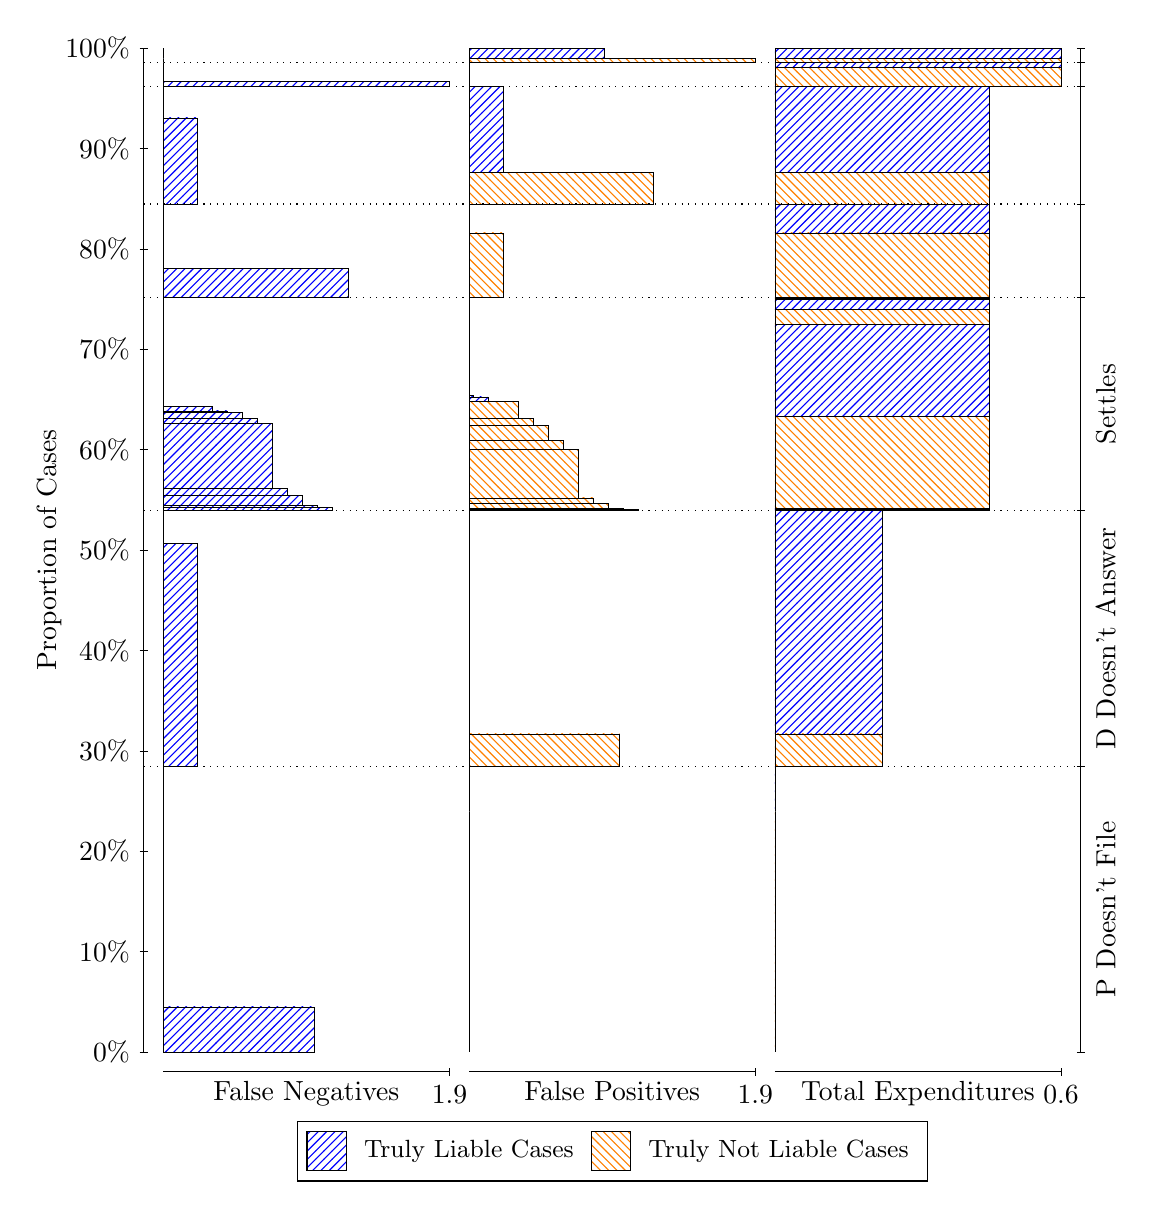
\begin{tikzpicture}
\draw[black, very thin] (1.5,1.75) -- (1.5,14.5);
\node[rotate=90, anchor=center] at (0.3, 8.125) {Proportion of Cases};
\draw[black, very thin] (1.45,1.75) -- (1.55,1.75);
\node[anchor=east] at (1.45, 1.75) {0\%};
\draw[black, very thin] (1.45,3.025) -- (1.55,3.025);
\node[anchor=east] at (1.45, 3.025) {10\%};
\draw[black, very thin] (1.45,4.3) -- (1.55,4.3);
\node[anchor=east] at (1.45, 4.3) {20\%};
\draw[black, very thin] (1.45,5.575) -- (1.55,5.575);
\node[anchor=east] at (1.45, 5.575) {30\%};
\draw[black, very thin] (1.45,6.85) -- (1.55,6.85);
\node[anchor=east] at (1.45, 6.85) {40\%};
\draw[black, very thin] (1.45,8.125) -- (1.55,8.125);
\node[anchor=east] at (1.45, 8.125) {50\%};
\draw[black, very thin] (1.45,9.4) -- (1.55,9.4);
\node[anchor=east] at (1.45, 9.4) {60\%};
\draw[black, very thin] (1.45,10.675) -- (1.55,10.675);
\node[anchor=east] at (1.45, 10.675) {70\%};
\draw[black, very thin] (1.45,11.95) -- (1.55,11.95);
\node[anchor=east] at (1.45, 11.95) {80\%};
\draw[black, very thin] (1.45,13.225) -- (1.55,13.225);
\node[anchor=east] at (1.45, 13.225) {90\%};
\draw[black, very thin] (1.45,14.5) -- (1.55,14.5);
\node[anchor=east] at (1.45, 14.5) {100\%};

\draw[black, very thin] (13.4,1.75) -- (13.4,14.5);
\draw[black, very thin] (13.35,1.75) -- (13.45,1.75);
\node[anchor=west] at (13.35, 1.75) {};
\draw[black, very thin] (13.35,5.3749) -- (13.45,5.3749);
\node[anchor=west] at (13.35, 5.3749) {};
\draw[black, very thin] (13.35,8.6261) -- (13.45,8.6261);
\node[anchor=west] at (13.35, 8.6261) {};
\draw[black, very thin] (13.35,11.334) -- (13.45,11.334);
\node[anchor=west] at (13.35, 11.334) {};
\draw[black, very thin] (13.35,12.519) -- (13.45,12.519);
\node[anchor=west] at (13.35, 12.519) {};
\draw[black, very thin] (13.35,14.016) -- (13.45,14.016);
\node[anchor=west] at (13.35, 14.016) {};
\draw[black, very thin] (13.35,14.315) -- (13.45,14.315);
\node[anchor=west] at (13.35, 14.315) {};
\draw[black, very thin] (13.35,14.5) -- (13.45,14.5);
\node[anchor=west] at (13.35, 14.5) {};

\draw[black, very thin, pattern color=blue, pattern=north east lines] (1.75,1.75) rectangle (3.6623,2.3213);
\draw[black, very thin, pattern color=orange, pattern=north west lines] (1.75,2.3213) rectangle (1.75,5.3749);
\draw[black, very thin, pattern color=blue, pattern=north east lines] (1.75,5.3749) rectangle (2.1803,8.2124);
\draw[black, very thin, pattern color=orange, pattern=north west lines] (1.75,8.2124) rectangle (1.75,8.6261);
\draw[black, very thin, pattern color=blue, pattern=north east lines] (1.75,8.6261) rectangle (3.9013,8.6652);
\draw[black, very thin, pattern color=blue, pattern=north east lines] (1.75,8.6652) rectangle (3.7101,8.6903);
\draw[black, very thin, pattern color=blue, pattern=north east lines] (1.75,8.6903) rectangle (3.5189,8.8156);
\draw[black, very thin, pattern color=blue, pattern=north east lines] (1.75,8.8156) rectangle (3.3276,8.9107);
\draw[black, very thin, pattern color=blue, pattern=north east lines] (1.75,8.9107) rectangle (3.1364,9.7338);
\draw[black, very thin, pattern color=blue, pattern=north east lines] (1.75,9.7338) rectangle (2.9452,9.7989);
\draw[black, very thin, pattern color=blue, pattern=north east lines] (1.75,9.7989) rectangle (2.7539,9.8742);
\draw[black, very thin, pattern color=blue, pattern=north east lines] (1.75,9.8742) rectangle (2.5627,9.8906);
\draw[black, very thin, pattern color=blue, pattern=north east lines] (1.75,9.8906) rectangle (2.3715,9.944);
\draw[black, very thin, pattern color=orange, pattern=north west lines] (1.75,9.944) rectangle (1.75,11.334);
\draw[black, very thin, pattern color=blue, pattern=north east lines] (1.75,11.334) rectangle (4.0925,11.701);
\draw[black, very thin, pattern color=orange, pattern=north west lines] (1.75,11.701) rectangle (1.75,12.519);
\draw[black, very thin, pattern color=blue, pattern=north east lines] (1.75,12.519) rectangle (2.1803,13.614);
\draw[black, very thin, pattern color=orange, pattern=north west lines] (1.75,13.614) rectangle (1.75,14.016);
\draw[black, very thin, pattern color=blue, pattern=north east lines] (1.75,14.016) rectangle (5.3833,14.072);
\draw[black, very thin, pattern color=orange, pattern=north west lines] (1.75,14.072) rectangle (1.75,14.315);
\draw[black, very thin, pattern color=orange, pattern=north west lines] (1.75,14.315) rectangle (1.75,14.37);
\draw[black, very thin, pattern color=blue, pattern=north east lines] (1.75,14.37) rectangle (1.75,14.5);
\draw[black, very thin, pattern color=orange, pattern=north west lines] (5.6333,1.75) rectangle (5.6333,4.8036);
\draw[black, very thin, pattern color=blue, pattern=north east lines] (5.6333,4.8036) rectangle (5.6333,5.3749);
\draw[black, very thin, pattern color=orange, pattern=north west lines] (5.6333,5.3749) rectangle (7.5456,5.7886);
\draw[black, very thin, pattern color=blue, pattern=north east lines] (5.6333,5.7886) rectangle (5.6333,8.6261);
\draw[black, very thin, pattern color=orange, pattern=north west lines] (5.6333,8.6261) rectangle (7.7846,8.6423);
\draw[black, very thin, pattern color=orange, pattern=north west lines] (5.6333,8.6423) rectangle (7.5934,8.6533);
\draw[black, very thin, pattern color=orange, pattern=north west lines] (5.6333,8.6533) rectangle (7.4022,8.7206);
\draw[black, very thin, pattern color=orange, pattern=north west lines] (5.6333,8.7206) rectangle (7.211,8.7863);
\draw[black, very thin, pattern color=orange, pattern=north west lines] (5.6333,8.7863) rectangle (7.0197,9.4073);
\draw[black, very thin, pattern color=orange, pattern=north west lines] (5.6333,9.4073) rectangle (6.8285,9.517);
\draw[black, very thin, pattern color=orange, pattern=north west lines] (5.6333,9.517) rectangle (6.6373,9.7125);
\draw[black, very thin, pattern color=orange, pattern=north west lines] (5.6333,9.7125) rectangle (6.4461,9.7961);
\draw[black, very thin, pattern color=orange, pattern=north west lines] (5.6333,9.7961) rectangle (6.2548,10.016);
\draw[black, very thin, pattern color=blue, pattern=north east lines] (5.6333,10.016) rectangle (5.8724,10.069);
\draw[black, very thin, pattern color=blue, pattern=north east lines] (5.6333,10.069) rectangle (5.6811,10.086);
\draw[black, very thin, pattern color=blue, pattern=north east lines] (5.6333,10.086) rectangle (5.6333,11.334);
\draw[black, very thin, pattern color=orange, pattern=north west lines] (5.6333,11.334) rectangle (6.0636,12.152);
\draw[black, very thin, pattern color=blue, pattern=north east lines] (5.6333,12.152) rectangle (5.6333,12.519);
\draw[black, very thin, pattern color=orange, pattern=north west lines] (5.6333,12.519) rectangle (7.9759,12.921);
\draw[black, very thin, pattern color=blue, pattern=north east lines] (5.6333,12.921) rectangle (6.0636,14.016);
\draw[black, very thin, pattern color=orange, pattern=north west lines] (5.6333,14.016) rectangle (5.6333,14.259);
\draw[black, very thin, pattern color=blue, pattern=north east lines] (5.6333,14.259) rectangle (5.6333,14.315);
\draw[black, very thin, pattern color=orange, pattern=north west lines] (5.6333,14.315) rectangle (9.2667,14.37);
\draw[black, very thin, pattern color=blue, pattern=north east lines] (5.6333,14.37) rectangle (7.3544,14.5);
\draw[black, very thin, pattern color=orange, pattern=north west lines] (9.5167,1.75) rectangle (9.5167,4.8036);
\draw[black, very thin, pattern color=blue, pattern=north east lines] (9.5167,4.8036) rectangle (9.5167,5.3749);
\draw[black, very thin, pattern color=orange, pattern=north west lines] (9.5167,5.3749) rectangle (10.879,5.7886);
\draw[black, very thin, pattern color=blue, pattern=north east lines] (9.5167,5.7886) rectangle (10.879,8.6261);
\draw[black, very thin, pattern color=orange, pattern=north west lines] (9.5167,8.6261) rectangle (12.242,8.6435);
\draw[black, very thin, pattern color=blue, pattern=north east lines] (9.5167,8.6435) rectangle (12.242,8.6516);
\draw[black, very thin, pattern color=orange, pattern=north west lines] (9.5167,8.6516) rectangle (12.242,9.8176);
\draw[black, very thin, pattern color=blue, pattern=north east lines] (9.5167,9.8176) rectangle (12.242,10.986);
\draw[black, very thin, pattern color=orange, pattern=north west lines] (9.5167,10.986) rectangle (12.242,11.181);
\draw[black, very thin, pattern color=blue, pattern=north east lines] (9.5167,11.181) rectangle (12.242,11.306);
\draw[black, very thin, pattern color=orange, pattern=north west lines] (9.5167,11.306) rectangle (12.242,11.317);
\draw[black, very thin, pattern color=blue, pattern=north east lines] (9.5167,11.317) rectangle (12.242,11.334);
\draw[black, very thin, pattern color=orange, pattern=north west lines] (9.5167,11.334) rectangle (12.242,12.152);
\draw[black, very thin, pattern color=blue, pattern=north east lines] (9.5167,12.152) rectangle (12.242,12.519);
\draw[black, very thin, pattern color=orange, pattern=north west lines] (9.5167,12.519) rectangle (12.242,12.921);
\draw[black, very thin, pattern color=blue, pattern=north east lines] (9.5167,12.921) rectangle (12.242,14.016);
\draw[black, very thin, pattern color=orange, pattern=north west lines] (9.5167,14.016) rectangle (13.15,14.259);
\draw[black, very thin, pattern color=blue, pattern=north east lines] (9.5167,14.259) rectangle (13.15,14.315);
\draw[black, very thin, pattern color=orange, pattern=north west lines] (9.5167,14.315) rectangle (13.15,14.37);
\draw[black, very thin, pattern color=blue, pattern=north east lines] (9.5167,14.37) rectangle (13.15,14.5);
\draw[black, dotted] (1.5,5.3749) -- (13.4,5.3749);
\draw[black, dotted] (1.5,8.6261) -- (13.4,8.6261);
\draw[black, dotted] (1.5,11.334) -- (13.4,11.334);
\draw[black, dotted] (1.5,12.519) -- (13.4,12.519);
\draw[black, dotted] (1.5,14.016) -- (13.4,14.016);
\draw[black, dotted] (1.5,14.315) -- (13.4,14.315);
\draw[black, very thin] (1.75,1.5) -- (5.3833,1.5);
\node[anchor=north] at (3.5667, 1.5) {False Negatives};
\draw[black, very thin] (5.3833,1.45) -- (5.3833,1.55);
\node[anchor=north] at (5.3833, 1.45) {1.9};

\draw[black, very thin] (5.6333,1.5) -- (9.2667,1.5);
\node[anchor=north] at (7.45, 1.5) {False Positives};
\draw[black, very thin] (9.2667,1.45) -- (9.2667,1.55);
\node[anchor=north] at (9.2667, 1.45) {1.9};

\draw[black, very thin] (9.5167,1.5) -- (13.15,1.5);
\node[anchor=north] at (11.333, 1.5) {Total Expenditures};
\draw[black, very thin] (13.15,1.45) -- (13.15,1.55);
\node[anchor=north] at (13.15, 1.45) {0.6};

\node[black, centered, rotate=90] at (13.72, 3.5624) {P Doesn't File};
\node[black, centered, rotate=90] at (13.72, 7.0005) {D Doesn't Answer};
\node[black, centered, rotate=90] at (13.72, 9.98) {Settles};





\draw (7.449999999999999,1.5) node[draw=none] (baseCoordinate) {};
\begin{scope}[align=center]
        \matrix[scale=0.5, draw=black, below=0.5cm of baseCoordinate, nodes={draw}, column sep=0.1cm]{
            \node[rectangle, draw, minimum width=0.5cm, minimum height=0.5cm, pattern=north east lines, pattern color=blue] {}; &
            \node[draw=none, font=\small] (B) {Truly Liable Cases}; &
            \node[rectangle, draw, minimum width=0.5cm, minimum height=0.5cm, pattern=north west lines, pattern color=orange] {}; &
            \node[draw=none, font=\small] (B) {Truly Not Liable Cases}; \\
            };
\end{scope}

\end{tikzpicture}
\end{document}